\chapter{Ring Homomorphisms and Isomorphisms}
Just like with groups, rings too have homomorphisms and isomorphisms, although they are defined slightly differently than in groups. Like how group homomorphisms preserve some structure between the two groups, ring homomorphisms and isomorphisms also preserve structure between rings.

\section{Ring Homomorphisms and Isomorphisms}
\begin{definition}
    Let $(R_1, +, \cdot)$ and $(R_2, \oplus, \otimes)$ be rings. A function $\phi: R_1 \to R_2$ is a \textbf{ring homomorphism}\index{ring homomorphism} if for all $a, b \in R_1$,
    \begin{align*}
        \phi(a+b) &= \phi(a) \oplus \phi(b), \text{ and}\\
        \phi(a\cdot b) &= \phi(a)\otimes\phi(b).
    \end{align*}
\end{definition}
\begin{remark}
    Like with group homomorphisms, we usually suppress the multiplication operation and use ``$+$'' for both addition operations. That is, the ring homomorphism conditions become
    \begin{align*}
        \phi(a+b) &= \phi(a) + \phi(b) \text{ and}\\
        \phi(ab) &= \phi(a)\phi(b).
    \end{align*}
\end{remark}

\begin{example}
    We show that the map $\phi: \Z \to \Z/n\Z, x \mapsto x + n\Z$ is a ring homomorphism.
     
    \begin{proof}
        Let $a, b \in \Z$. Note
        \begin{align*}
            \phi(a+b) &= (a+b) + n\Z\\
            &= (a + n\Z) + (b + n\Z) & (\text{Definition of coset addition})\\
            &=\phi(a)+\phi(b)
        \end{align*}
        and
        \begin{align*}
            \phi(ab) &= (ab) + n\Z\\
            &= (a + n\Z)(b + n\Z) & (\text{Definition of coset multiplication})\\
            &= \phi(a)\phi(b)
        \end{align*}
        so $\phi$ is a homomorphism.
    \end{proof}
\end{example}

\begin{example}
    Consider
    \[
        R = \left\{\begin{pmatrix}a&b\\0&c\end{pmatrix}\vert a,b,c\in\Z\right\}.
    \]
    Let $\phi: R \to \Z^2, \begin{pmatrix}a&b\\0&c\end{pmatrix} \mapsto (a,c)$. We show that $\phi$ is a ring homomorphism.

    \begin{proof}
        We see that
        \begin{align*}
            \phi\left(\begin{pmatrix}a&b\\0&c\end{pmatrix} + \begin{pmatrix}x&y\\0&z\end{pmatrix}\right) &= \phi\left(\begin{pmatrix}a+x&b+y\\0&c+z\end{pmatrix}\right)\\
            &= (a+x,c+z)\\
            &= (a,c) + (x,z)\\
            &= \phi\left(\begin{pmatrix}a&b\\0&c\end{pmatrix}\right) + \phi\left(\begin{pmatrix}x&y\\0&z\end{pmatrix}\right)
        \end{align*}
        and also
        \begin{align*}
            \phi\left(\begin{pmatrix}a&b\\0&c\end{pmatrix}\begin{pmatrix}x&y\\0&z\end{pmatrix}\right) &= \phi\left(\begin{pmatrix}ax&ay+bz\\0&cz\end{pmatrix}\right)\\
            &= (ax, cz)\\
            &= (a,c)(x,z)\\
            &= \phi\left(\begin{pmatrix}a&b\\0&c\end{pmatrix}\right)\phi\left(\begin{pmatrix}x&y\\0&z\end{pmatrix}\right)
        \end{align*}
        so $\phi$ is a homomorphism.
    \end{proof}
\end{example}
\begin{exercise}
    Let $\phi: \Mn{2}{\Z} \to \Z$ be such that
    \[
        \phi\left(\begin{pmatrix}a&b\\c&d\end{pmatrix}\right) = a+d.
    \]
    Is $\phi$ a ring homomorphism?
\end{exercise}

An endomorphism is a specific type of homomorphism.
\begin{definition}
    Let $R$ be a ring. A \textbf{ring endomorphism}\index{ring endomorphism} of $R$ is a homomorphism $\phi: R \to R$.
\end{definition}
\begin{example}
    Let $R$ be a commutative ring with prime characteristic $p$. The \textbf{Frobenius endomorphism}\index{Frobenius endomorphism} $\phi: R \to R$ is such that $\phi(r) = r^p$. We show that $\phi$ is a ring endomorphism.
    
    \begin{proof}
        Note that
        \begin{align*}
            \phi(a+b) &= (a+b)^p\\
            &= a^p + pa^{p-1}b + {p \choose 2}a^{p-2}b^2 + \cdots + pab^{p-1} + b^p.
        \end{align*}
        Note that the binomial coefficients ${p \choose k}$ where $1 \leq k \leq p -1$ are all multiples of $p$. As the characteristic of the ring $R$ is $p$, thus $px = 0$ for any $x \in R$. Therefore,
        \begin{align*}
            \phi(a+b) = &a^p + pa^{p-1}b + {p \choose 2}a^{p-2}b^2 + \cdots + pab^{p-1} + b^p\\
            &= a^p + 0 + 0 + \cdots + 0 + b^p\\
            &= a^p + b^p\\
            &=\phi(a) + \phi(b)
        \end{align*}

        Also,
        \[
            \phi(ab) = (ab)^p = a^pb^p = \phi(a)\phi(b).
        \]
        Therefore $\phi$ is a ring endomorphism.
    \end{proof}
\end{example}

\begin{exercise}
    Let $R$ be a ring and $\phi: R \to R$ is a map. Show that $\phi$ is a ring endomorphisms in the following cases.
    \begin{partquestions}{\alph*}
        \item $\phi(r) = 0$ (the \textbf{trivial homomorphism}\index{trivial homomorphism})
        \item $\phi(r) = r$ (the \textbf{identity homomorphism}\index{identity homomorphism})
    \end{partquestions}
\end{exercise}

Similar to group isomorphisms, rings too have an analogous `isomorphism' definition.
\begin{definition}
    A \textbf{ring isomorphism}\index{ring isomorphism} is a bijective ring homomorphism.
\end{definition}
Similar to groups, if two rings $R$ and $R'$ are isomorphic, then we write $R \cong R'$.

\begin{example}
    We show that $\Z_n \cong \Z/n\Z$.

    \begin{proof}
        Consider the map $\phi:\Z_n \to \Z/n\Z$ where $m \mapsto m + n\Z$. We show that $\phi$ is an isomorphism.
        \begin{itemize}
            \item \textbf{Homomorphism}:
            \[
                \phi(a+b) = (a+b) + n\Z = (a + n\Z) + (b + n\Z) = \phi(a) + \phi(b)
            \]
            and
            \[
                \phi(ab) = (ab) + n\Z = (a+n\Z)(b+n\Z) = \phi(a)\phi(b)
            \]

            \item \textbf{Injective}: Suppose $a, b \in \Z_n$ such that $\phi(a) = \phi(b)$. This means $a + n\Z = b + n\Z$. Now note that $0 \leq a,b < n$ so we have $a = b$.
            
            \item \textbf{Surjective}: Suppose $m + n\Z \in \Z/n\Z$. Applying Euclid's division lemma (\myref{lemma-euclid-division}) on $m$ we have
            \[
                m = nq + r
            \]
            with $0 \leq r < n$. One sees that
            \begin{align*}
                \phi(r) &= r + n\Z\\
                &= r + (nq + n\Z)\\
                &= (r + nq) + n\Z\\
                &= m + n\Z
            \end{align*}
            so $m + n\Z$ has a pre-image of $r$ in $\Z_n$.
        \end{itemize}
        Since $\phi$ is a bijective ring homomorphism, this $\phi$ is an isomorphism, meaning $\Z_n \cong \Z/n\Z$ as rings.
    \end{proof}
\end{example}
\begin{example}
    We show that $\Z \not\cong 2\Z$ as rings.

    \begin{proof}
        Suppose $\phi: \Z \to 2\Z$ is a ring isomorphism.

        Set $a = \phi(1) = 2\Z$. Note that
        \[
            a = \phi(1) = \phi(1\times1) = (\phi(1))^2 = a^2
        \]
        so $a^2 = a$, which means $a = 0$ or $a = 1$. But as $a \in 2\Z$, thus $a \neq 1$ which means $a = 0$.

        Now notice for any $n \in \Z$ we have
        \begin{align*}
            \phi(n) &= \phi(n1)\\
            &= \phi(n)\phi(1)\\
            &= \phi(n) \times 0\\
            &= 0.
        \end{align*}
        Thus one sees that $\phi(0) = \phi(1) = 0$ which means $\phi$ is not injective, a contradiction.
    \end{proof}
\end{example}
\begin{exercise}\label{exercise-identity-homomorphism-is-an-isomorphism}
    Show that the identity homomorphism is an isomorphism.
\end{exercise}

\section{Properties of Ring Homomorphisms}
For the following, let $R_1$ and $R_2$ be rings, and $\phi: R_1 \to R_2$ be a ring homomorphism.

\begin{exercise}\label{exercise-image-of-additive-identity-is-additive-identity}
    Show $\phi(0_1) = 0_2$, where $0_1$ is the additive identity of $R_1$ and $0_2$ is the additive identity of $R_2$.
\end{exercise}

\begin{exercise}
    Suppose $R_1$ and $R_2$ are division rings. Show $\phi(1_1) = 1_2$, where $1_1$ is the multiplicative identity of $R_1$ and $1_2$ is the multiplicative identity of $R_2$.
\end{exercise}

\begin{exercise}
    Let $x \in R_1$.
    \begin{partquestions}{\alph*}
        \item Show that $\phi(-x) = -\phi(x)$.
        \item If $R_1$ and $R_2$ are division rings, show that $\phi(x^{-1}) = (\phi(x))^{-1}$.
    \end{partquestions}
\end{exercise}

\begin{proposition}\label{prop-homomorphism-on-subring-is-subring}
    If $S$ is a subring of $R_1$, then
    \[
        \phi(S) = \{\phi(s) | s \in S\}
    \]
    is a subring of $R_2$.
\end{proposition}
\begin{proof}
    Let $S$ be a subring of $R_1$. Take $a, b \in \phi(S)$, which means that there exist $s_a$ and $s_b$ such that $\phi(s_a) = a$ and $\phi(s_b) = b$.
    \begin{itemize}
        \item We show that $(\phi(S), +) \leq (R_2, +)$.
        \begin{itemize}
            \item $\phi(S) \neq \emptyset$ since $\phi(0_1) = 0_2 \in \phi(S)$.
            \item $a - b = \phi(s_a) - \phi(s_b) = \phi(s_a-s_b) \in \phi(S)$.
        \end{itemize}

        \item Now we show $ab \in \phi(S)$.
        \[
            ab = \phi(s_a)\phi(s_b) = \phi(s_as_b) \in \phi(S).
        \]
    \end{itemize}
    Therefore $\phi(S)$ is a subring of $R_2$.
\end{proof}

\begin{proposition}
    If $\phi$ is surjective and $I$ is an ideal of $R_1$, then $\phi(I)$ is an ideal of $R_2$.
\end{proposition}
\begin{proof}
    From previous proposition $\phi(I)$ is a subring of $R_2$. We just need to show that $\phi(I)$ is an ideal of $R_2$.

    Take $a \in \phi(I)$ and $r_2 \in R_2$. As $\phi$ is surjective, we can find a $r_1 \in R_1$ such that $\phi(r_1) = r_2$. Also, let $a = \phi(i)$ for an $i \in I$.

    Note
    \begin{align*}
        ar_2 = \phi(i)\phi(r_1) = \phi(\underbrace{ir_1}_{\text{In }I}) \in \phi(I)\\
        r_2a = \phi(r_1)\phi(i) = \phi(\underbrace{r_1i}_{\text{In }I}) \in \phi(I)
    \end{align*}
    so $\phi(I)$ is an ideal of $R_2$.
\end{proof}

\begin{proposition}\label{prop-inverse-homomorphism-on-ideal-is-ideal}
    Let $J$ be an ideal of $R_2$. Then
    \[
        \phi^{-1}(J) = \{r \in R_1 \vert \phi(r) \in J\}
    \]
    is an ideal of $R_1$.
\end{proposition}
\begin{proof}
    Suppose $J$ is an ideal of $R_2$. We consider the test for ideal (\myref{thrm-test-for-ideal}) to show $\phi^{-1}(J)$ is an ideal of $R_1$.
    
    One sees that $\phi^{-1}(J) \neq \emptyset$ since $\phi(0_1) = 0_2 \in J$, so $0_1 \in \phi^{-1}(J)$.

    Let $a, b \in \phi^{-1}(J)$, so $\phi(a), \phi(b) \in J$. Note that
    \[
        \phi(a-b) = \phi(a) - \phi(b) \in J
    \]
    so $a-b \in \phi^{-1}(J)$ for all $a,b \in J$.

    Let $r \in R_1$ and $a \in \phi^{-1}(J)$. Note that $\phi(a) \in J$ and $\phi(r) \in R_2$, so
    \begin{align*}
        \underbrace{\phi(a)}_{\text{In }J}\underbrace{\phi(r)}_{\text{In }R_2} &\in J & (J\text{ is an ideal, so } rj \in J)\\
        \phi(r)\phi(a) &\in J & (\text{since } jr \in J).
    \end{align*}
    Note $\phi(a)\phi(r) = \phi(ar) \in J$, so $ar \in \phi^{-1}(J)$, and similarly we have $\phi(r)\phi(a) = \phi(ra) \in J$, so $ra \in \phi^{-1}(J)$.

    Therefore, by the test for ideal, is an ideal of $R_1$.
\end{proof}

\section{Image and Kernel}
Similar to groups, ring homomorphisms too have a image and kernel.
\begin{definition}
    The \textbf{image}\index{image} of a ring homomorphism $\phi: R_1 \to R_2$ is $\im\phi = \{\phi(r) \vert r \in R_1\}$.
\end{definition}
\begin{definition}
    The \textbf{kernel}\index{kernel} of a ring homomorphism $\phi:R_1 \to R_2$ is $\ker\phi = \{r \in R_1 \vert \phi(r) = 0\}$.
\end{definition}

\begin{example}\label{example-homomorphism-on-upper-triangle-matrices}
    Consider the ring
    \[
        R = \left\{\begin{pmatrix}a&b\\0&c\end{pmatrix}\vert a,b,c\in\Z\right\}.
    \]
    and the homomorphism $\phi: R \to \Z^2, \begin{pmatrix}a&b\\0&c\end{pmatrix} \mapsto (a,c)$.

    We note that $\phi$ is surjective; for any $(x,y)\in\Z^2$, we note that $\phi\left(\begin{pmatrix}x&0\\0&y\end{pmatrix}\right) = (x,y)$ so $(x,y)$ has a pre-image in $R$. Therefore $\im \phi = \Z^2$.

    We now find the kernel of $\phi$.
    \begin{align*}
        \ker\phi &= \left\{\begin{pmatrix}a&b\\0&c\end{pmatrix} \in R \vert \phi\left(\begin{pmatrix}a&b\\0&c\end{pmatrix}\right) = (0,0)\right\}\\
        &= \left\{\begin{pmatrix}a&b\\0&c\end{pmatrix} \in R \vert (a,c) = (0,0)\right\}\\
        &= \left\{\begin{pmatrix}0&n\\0&0\end{pmatrix} \vert n \in \Z\right\}.
    \end{align*}
\end{example}

We look at some results regarding the image and kernel of a ring homomorphism. These results may look familiar to those who read Volume I.
\begin{proposition}\label{prop-image-is-a-subring}
    Let $R_1$ and $R_2$ be rings, and let $\phi: R_1 \to R_2$ be a ring homomorphism. Then $\im\phi$ is a subring of $R_2$.
\end{proposition}
\begin{proof}
    Note that $\im\phi = \phi(R_1)$ is a subring of $R_2$ by \myref{prop-homomorphism-on-subring-is-subring}.
\end{proof}

\begin{proposition}\label{prop-kernel-is-an-ideal}
    Let $R_1$ and $R_2$ be rings, and let $\phi: R_1 \to R_2$ be a ring homomorphism. Then $\ker\phi$ is an ideal of $R_1$.
\end{proposition}
\begin{proof}
    See \myref{exercise-kernel-is-an-ideal} (later).
\end{proof}
\begin{exercise}\label{exercise-kernel-is-an-ideal}
    Let $R_1$ and $R_2$ be rings, and let $\phi: R_1 \to R_2$ be a ring homomorphism. Prove that $\ker\phi$ is an ideal of $R_1$.
\end{exercise}

\begin{proposition}
    Let $R_1$ and $R_2$ be rings, and let $\phi: R_1 \to R_2$ be a ring homomorphism. Then $\phi$ is injective if and only if $\ker\phi = \{0_1\}$.
\end{proposition}
\begin{proof}
    We first prove the forward direction; suppose $\phi$ is injective and let $a \in \ker\phi$. By definition of the kernel we have $\phi(a) = 0_2$. But by \myref{exercise-image-of-additive-identity-is-additive-identity}, we have $\phi(0_1) = 0_2$. Since $\phi$ is injective, therefore $a = 0_1$, meaning $\ker\phi = \{0_1\}$.

    We now prove the reverse direction; suppose $\ker\phi = \{0_1\}$. Now let $a,b \in R_1$ such that $\phi(a) = \phi(b)$. Therefore $\phi(a) - \phi(b) = \phi(a-b) = 0_2$. Therefore $a-b \in \ker\phi$ by definition of the kernel. However $\ker\phi = \{0_1\}$ which means that $a - b = 0_1$. Therefore $a = b$, meaning $\phi$ is injective.
\end{proof}

\section{The Ring Isomorphism Theorems}
Similar to group theory, there are three main ring isomorphism theorems. However, we will only explicitly prove the first ring isomorphism theorem; the other two will be left as problems.

\begin{theorem}[First Ring Isomorphism Theorem (FRIT)]\label{thrm-ring-isomorphism-1}\index{ring isomorphism theorem!first}\index{FRIT}
    Let $R$ and $R'$ be rings, and suppose $\phi: R \to R'$ is a ring homomorphism. Then the map $\psi: R / \ker\phi \to \im\phi$, defined by $\psi(r + \ker\phi) = \phi(r)$, is a ring isomorphism.
\end{theorem}
\begin{remark}
    Equivalently, the FRIT states that
    \[
        R / \ker\phi \cong \im\phi
    \]
    for any ring homomorphism $\phi$.
\end{remark}

\newpage

We include the commutativity diagram of the maps stated to aid clarity:
\begin{figure}[h]
    \centering
    \fbox{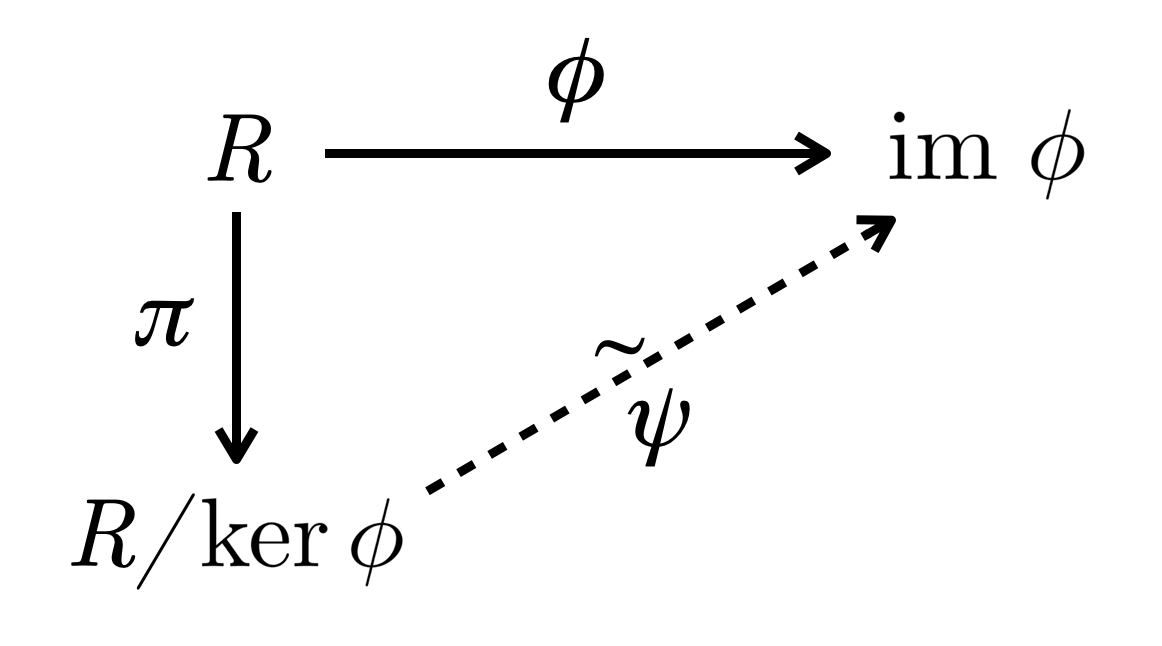
\includegraphics[width=4.5cm]{ring-homomorphisms/iso-1-comm-diagram.png}}
    \caption{Commutativity Diagram for \myreffigures{thrm-ring-isomorphism-1}}
\end{figure}

In the diagram, $\phi$ sends elements from $R$ to $\im\phi$ and $\pi$ sends elements from $R$ to $R/\ker\phi$. Then the map $\psi$ is a unique map that sends elements from $R/\ker\phi$ to the image of $\phi$.

\begin{proof}
    We need to show that $\psi$ is a well-defined bijective ring homomorphism.
    \begin{itemize}
        \item \textbf{Well-Defined}: Suppose $a + \ker\phi$ and $b + \ker\phi$ are in $R/\ker\phi$ such that $a + \ker\phi = b+\ker\phi$. This means that $a - b \in \ker\phi$ by Coset Equality (\myref{lemma-coset-equality}). Thus $\phi(a-b) = 0$ by definition of the kernel. Hence $\phi(a) - \phi(b) = 0$ which means $\phi(a) = \phi(b)$. Therefore, we see that
        \[
            \psi(a + \ker\phi) = \phi(a) = \phi(b) = \psi(b + \ker\phi)
        \]
        which means $\psi$ is well-defined.

        \item \textbf{Homomorphism}: We first show that $\psi$ is a ring homomorphism.
        \begin{itemize}
            \item $\boxed{+}$: If $a + \ker\phi$ and $b + \ker\phi$ are in $R/\ker\phi$,
            \begin{align*}
                &\psi((a + \ker\phi)+(b+\ker\phi))\\
                &= \psi((a+b)+\ker\phi)\\
                &= \phi(a+b)\\
                &= \phi(a) + \phi(b)\\
                &= \psi(a + \ker\phi) + \psi(b + \ker\phi).
            \end{align*}
            \item $\boxed{\times}$: If $a + \ker\phi$ and $b + \ker\phi$ are in $R/\ker\phi$,
            \begin{align*}
                \psi((a + \ker\phi)(b+\ker\phi)) &= \psi((ab)+\ker\phi)\\
                &= \phi(ab)\\
                &= \phi(a)\phi(b)\\
                &= \psi(a + \ker\phi)\psi(b + \ker\phi).
            \end{align*}
        \end{itemize}
        Therefore $\psi$ is a ring homomorphism.

        \item \textbf{Injective}: Suppose $\psi(a+\ker\phi) = \psi(b+\ker\phi)$.
        \begin{align*}
            \phi(a) &= \phi(b) & (\text{definition of }\psi)\\
            \phi(a) - \phi(b) &= 0\\
            \phi(a-b) &= 0 & (\phi \text{ is a ring homomorphism})\\
            a - b &\in \ker\phi & (\text{definition of kernel})\\
            a + \ker\phi &= b + \ker\phi & (\text{Coset Equality})
        \end{align*}
        Therefore if $\psi(a+\ker\phi) = \psi(b+\ker\phi)$ then $a+\ker\phi = b+\ker\phi$, which means $\psi$ is injective.

        \item \textbf{Surjective}: Suppose $s \in \im\phi$, so there is an $r \in R$ such that $s = \phi(r)$. Clearly $\psi(r + \ker\phi) = \phi(r) = s$, so $s$ has a pre-image of $r + \ker\phi$, i.e. $\psi$ is surjective.
    \end{itemize}
    Therefore, $\psi$ is a bijective ring homomorphism, i.e. $\psi$ is a ring isomorphism, proving the FRIT.
\end{proof}

\begin{example}
    Consider the ring
    \[
        R = \left\{\begin{pmatrix}a&b\\0&c\end{pmatrix}\vert a,b,c\in\Z\right\}
    \]
    and the homomorphism $\phi: R \to \Z^2, \begin{pmatrix}a&b\\0&c\end{pmatrix} \mapsto (a,c)$. We found in \myref{example-homomorphism-on-upper-triangle-matrices} that $\phi$ is surjective (i.e., $\im\phi = \Z^2$) with kernel
    \[
        \left\{\begin{pmatrix}0&n\\0&0\end{pmatrix} \vert n \in \Z\right\}
    \]
    which, for brevity, we shall denote by $I$. Then, we see via the FRIT (\myref{thrm-ring-isomorphism-1}) that
    \[
        R/I \cong \Z^2.
    \]
\end{example}
\begin{exercise}
    Show that $\Z_n \cong \Z/n\Z$ via the ring homomorphism
    \[
        \phi: \Z \to \Z_n, m \mapsto m \mod n
    \]
    and by using the FRIT.
\end{exercise}

\newpage

We briefly mention the other two main ring isomorphism theorems, although the proof of them will be left as problems. They are much less used than the FRIT, so we make only a passing mention of them.
\begin{theorem}[Second Ring Isomorphism Theorem]\label{thrm-ring-isomorphism-2}\index{ring isomorphism theorem!second}
    Let $R$ be a ring with subring $R$ and ideal $I$. Then
    \begin{enumerate}
        \item $S+I = \{s+i \vert s\in S,\;i\in I\}$ is a subring of $R$;
        \item $S \cap I$ is an ideal of $S$; and
        \item $(S+I)/I \cong S/(S\cap I)$.
    \end{enumerate}
\end{theorem}
\begin{proof}
    See \myref{problem-ring-isomorphism-2} (later).
\end{proof}

\begin{theorem}[Third Ring Isomorphism Theorem]\label{thrm-ring-isomorphism-3}\index{ring isomorphism theorem!third}
    Let $R$ be a ring with ideals $I$ and $J$ such that $I$ is a subset of $J$. Then
    \begin{enumerate}
        \item $J/I$ is an ideal of $R/I$; and
        \item $\frac{R/I}{J/I} \cong R/J$.
    \end{enumerate}
\end{theorem}
\begin{proof}
    See \myref{problem-ring-isomorphism-3} (later).
\end{proof}

\newpage

\section{How Restrictive are Ring Homomorphisms?}
Although ring homomorphisms appear to be quite general, we explore how restricted they really are when dealing with certain rings.

\begin{example}\label{example-endomorphisms-of-Z}
    We find all ring endomorphisms of $\Z$.

    Let $\phi:\Z\to\Z$ be a ring endomorphism. Set $a = \phi(1)$. Note that
    \[
        a = \phi(1) = \phi(1\times1) = \phi(1)\phi(1) = a^2
    \]
    so $a^2 = a$. Thus $a = 0$ or $a = 1$ in $\Z$.

    If $a = 0$, then for any $n \in \Z$ we have
    \[
        \phi(n) = \phi(1n) = \phi(1)\phi(n) = 0\phi(n) = 0
    \]
    so $\phi(n) = 0$ for all $n \in \Z$, which is the trivial homomorphism.

    Now consider the case that $a = 1$. We claim that $\phi(n) = n$ for all $n \in \Z$.

    We leave the proof that $\phi(n) = n$ for all \textit{positive} integers $n$ for \myref{exercise-homomorphism-maps-n-to-n-if-n-is-positive} (later). Furthermore $\phi(0) = 0$ by the properties of ring homomorphism (specifically \myref{exercise-image-of-additive-identity-is-additive-identity}). Finally, note that for any non-negative integer $n$,
    \begin{align*}
        0 = \phi(0) &= \phi(n - n)\\
        &= \phi(n) + \phi(-n)\\
        &= n + \phi(-n)
    \end{align*}
    which means $\phi(-n) = -n$. Therefore $\phi(n) = n$ for all integers $n$.

    Therefore, the only ring endomorphisms $\phi:\Z\to\Z$ are $\phi(n) = 0$ or $\phi(n) = n$ for all integers $n$.
\end{example}
\begin{exercise}\label{exercise-homomorphism-maps-n-to-n-if-n-is-positive}
    In the above example, show that $\phi(n) = n$ for all positive integers $n$.
\end{exercise}
Note that in \myref{example-endomorphisms-of-Z} we started the entire computation with the observation that $\phi(1) = \phi(1)^2$. This means that $\phi(1)$ is an idempotent.
\begin{definition}
    Let $R$ be a ring. Then an element $x$ in $R$ is an \textbf{idempotent}\index{idempotent} if and only if $x^2 = x$.
\end{definition}
\begin{proposition}\label{prop-homomorphism-on-multiplicative-identity-is-idempotent}
    Let $R$ and $R'$ be rings, and let $\phi: R \to R'$ be a ring homomorphism. If $R$ is a ring with identity, then $\phi(1)$ is an idempotent.
\end{proposition}
\begin{proof}
    Note
    \[
        \phi(1) = \phi(1 \times 1) = \phi(1) \times \phi(1) = \left(\phi(1)\right)^2
    \]
    which means $\phi(1)$ is an idempotent.
\end{proof}

In \myref{example-endomorphisms-of-Z} we used the fact that the only idempotents of $\Z$ are 0 and 1. However, this is not true for all rings.

\begin{example}\label{example-homomorphisms-from-Z12-to-Z28}
    We find all ring homomorphisms $\phi: \Z_{12} \to \Z_{28}$. Note that $\Z_{12}$ is a ring with identity.

    By \myref{prop-homomorphism-on-multiplicative-identity-is-idempotent}, $a = \phi(1)$ is an idempotent. However, we cannot just assume that 0 and 1 are the \textit{only} idempotents in $\Z_{28}$; we need to check for them exhaustively.

    \newpage

    By exhaustion, we see that
    \begin{itemize}
        \item $0^2 = 0$;
        \item $1^2 = 1$;
        \item $8^2 = 64 = 2 \times 28 + 8 = 8$; and
        \item $21^2 = 441 = 15 \times 28 + 21 = 21$.
    \end{itemize}
    So the idempotents in $\Z_{28}$ are 0, 1, 8, and 21. This is not enough to narrow down the possible values of $\phi(1)$, so we need to invoke more facts.

    Recall from Volume I that $|\phi(1)|_+$ divides $|1|_+$ by \myref{exercise-order-of-homomorphism-divides-order}. Therefore $|\phi(1)|_+$ divides 12. Furthermore, \myref{thrm-order-of-element-in-cyclic-group} tells us that the additive order of an element $k$ in the group $(\Z_n, +)$ is $\frac{n}{\gcd(k,n)}$. So we must now exhaust all idempotents in $\Z_{28}$ to check whether it is a valid value of $\phi(1)$.
    \begin{itemize}
        \item $|0|_+ = 1$ which clearly divides 12, so it is a valid value of $\phi(1)$.
        \item $|1|_+ = 28$ which does not divide 12, so it is not a valid value of $\phi(1)$. This is one way that differs from the previous example, where 1 \textit{was} a possible value of $\phi(1)$.
        \item $|8|_+ = \frac{28}{\gcd(8,28)} = \frac{28}4 = 7$ which does not divide 12, so it is not a valid value of $\phi(1)$.
        \item $|21|_+ = \frac{28}{\gcd(21,28)} = \frac{28}7 = 4$ which divides 12, so it is a valid value of $\phi(1)$.
    \end{itemize}
    Hence $a \in \{0, 21\}$, i.e. $\phi(1) = 0$ or $\phi(1) = 21$.

    If $\phi(1) = 0$, then for any $n \in \Z_{12}$,
    \begin{align*}
        \phi(n) &= \phi(\underbrace{1 + 1 + \cdot + 1}_{n \text{ times}})\\
        &= \underbrace{\phi(1) + \phi(1) + \cdot + \phi(1)}_{n \text{ times}}\\
        &= \underbrace{0 + 0 + \cdots + 0}_{n \text{ times}}\\
        &= 0
    \end{align*}
    which means that $\phi(n) = 0$ for all $n \in \Z_{12}$, i.e. $\phi$ is trivial.

    If instead $\phi(1) = 21$, then
    \begin{align*}
        \phi(n) &= \underbrace{\phi(1) + \phi(1) + \cdot + \phi(1)}_{n \text{ times}}\\
        &= \underbrace{21 + 21 + \cdots + 21}_{n \text{ times}}\\
        &= 21n
    \end{align*}
    which means $\phi(n) = 21n$ for all $n \in \Z_{12}$.

    Thus the only homomorphisms $\phi: \Z_{12} \to \Z_{28}$ are $\phi(n) = 0$ and $\phi(n) = 21n$ for all $n \in \Z_{12}$.
\end{example}

\begin{exercise}\label{exercise-homomorphism-over-Q-fixes-elements-of-Q}
    Suppose $R$ and $R'$ are rings such that $\Q$ is a subring of both $R$ and $R'$. Let $\phi: R \to R'$ be a ring homomorphism such that $\phi(1) = 1$. Show that for any $q \in Q$ we have $\phi(q) = q$.
\end{exercise}

\newpage

\section{Problems}
\begin{problem}
    Let $R$ be a ring.
    \begin{partquestions}{\roman*}
        \item Show that $R/\{0\} \cong R$.
        \item Prove that $R$ is an integral domain if and only if $\{0\}$ is a prime ideal.
        \item Prove that $R$ is a field if and only if $\{0\}$ is a maximal ideal.
    \end{partquestions}
\end{problem}

\begin{problem}
    Find all ring endomorphisms of $\Q$.
\end{problem}

\begin{problem}
    Show $\Z^2 \not\cong \Q$.
\end{problem}

\begin{problem}
    Show $\Q[\sqrt2] \not\cong \Q[\sqrt3]$.
\end{problem}

\begin{problem}
    Let
    \[
        R = \left\{\begin{pmatrix}a&0\\0&b\end{pmatrix}\vert a,b \in \Z\right\},
    \]
    which is a subring of $\Mn{2}{\Z}$. Show that $R \cong \Z^2$.
\end{problem}

\begin{problem}
    Let $R$ and $R'$ be rings, and let $\phi: R \to R'$ be a ring isomorphism. Prove or disprove the following statements.
    \begin{partquestions}{\alph*}
        \item $\phi^{-1}: R' \to R$ is a ring isomorphism.
        \item If $R$ has a subring with $n$ elements, then so does $R'$.
        \item If $R$ has an ideal, then so does $R'$.
    \end{partquestions}
\end{problem}

\begin{problem}
    Find all ring endomorphisms of $\Z_{10}$.\newline
    Hence find all ring isomorphisms $\psi: \Z_{10} \to \Z_{10}$.
\end{problem}

\begin{problem}
    Find all endomorphisms over $\Q[\sqrt3]$.\newline
    Hence find all ring isomorphisms $\psi: \Q[\sqrt3] \to \Q[\sqrt3]$.
\end{problem}

\begin{problem}
    Let $R$ and $R'$ be commutative rings, $I$ be an ideal of $R$, and $\phi: R\to R'$ be a ring homomorphism.
    \begin{partquestions}{\roman*}
        \item Show that $\phi(\sqrt I) \subseteq \sqrt{\phi(I)}$.
        \item If $\phi$ is surjective with $\ker\phi \subseteq I$, prove that $\phi(\sqrt I) = \sqrt{\phi(I)}$.
    \end{partquestions}
\end{problem}

\begin{problem}\label{problem-ring-isomorphism-2}
    Let $R$ be a ring with subring $S$ and ideal $I$.
    \begin{partquestions}{\roman*}
        \item Prove $S+I$ is a subring of $R$.
        \item Prove $S \cap I$ is an ideal of $S$.
        \item Prove $S/(S\cap I)\cong (S+I)/I$.
    \end{partquestions}
\end{problem}

\begin{problem}\label{problem-ring-isomorphism-3}
    Let $R$ be a ring with ideals $I$ and $J$ such that $I$ is a subset of $J$.
    \begin{partquestions}{\roman*}
        \item Prove that $J/I$ is an ideal of $R/I$.
        \item Prove that $\frac{R/I}{J/I} \cong R/J$.\newline
        (\textit{Note: remember to prove that the map is well-defined.})
    \end{partquestions}
\end{problem}
